A statistical analysis is carried out to estimate the sensitivity to SMEFT effects in Higgs boson interactions of the STXS measurements compared to that of a dedicated analysis using a multivariate classifier. To this affect, a simple significance analysis is used based on the {\sc RooStats} framework~\cite{Moneta:2010pm} which determines the expected signifiance using an asymptotic calculator with nominal Asimov data sets and a one-sided profile likelihood. 

Naturally, a few approximations have been made. No systematic uncertainties have been considered, even if the generated events have been smeared to reflect the limited resolution and corrected for the finite efficiencies of $b$-tagging. The measurement in the STXS bins requires an extrapolation from the measured phase, which includes those selections applied specifically to reject backgrounds, in this case from the $Z b\bar{b}$ background. In case of the present analysis this is achieved using a BDT specifically trained to select $H\to b\bar{b}$ over $Z b\bar{b}$ events. For the STXS analysis, a BDT cut of $<$0.1 is applied, retaining 18.6\% of all SM Higgs events but less than 1\% of the $Z b\bar{b}$ background. For the BDT analysis targeting EFT operators, two settings are explored: Using the same BDT requirement as in the STXS analysis and additionally using a selection requirement of the BDT of $<$0.055 (and 0.06 for $c_{\sss HW} <0$) which leads to similar acceptances as in the STXS case. 

In a real-life analysis, the effects of using the BDT-selection would have to be accounted for. Herein, it is assumed, that these are perfectly known for both SM and BSM events with $c_{\sss HW} \neq 0$. Different acceptances of SM and BSM however can play a role, when testing for BSM physics in the STXS phase space, to which the events selected on detector level have been extrapolated assuming the SM acceptances alone. For information, the acceptances of the BDT-selection for both, SM and BSM events with $c_{\sss HW} \neq 0$ are summarized in Table~\ref{tab:bkg_acceptance}. The same applies to a dedicated SMEFT analysis as presented here: The acceptance of the first BDT selection needs to be modelled well as also the BDT classifier distribution used to constrain the BSM SMEFT phase space. The acceptance of the first BDT selection is summarized in Table~\ref{tab:bkg_acceptance}. The acceptance for the SM Higgs can (depending on the BDT cut) be indeed very similar for both STXS BDT and EFT optimized-BDT (around 18\%). The acceptance for events with a Wilson coefficent $c_{\sss HW}=0.3$ is larger than that by about a factor of 1.5 whilst it is smaller by the 25\% for $c_{\sss HW}=-0.3$. For the samples produced with a smaller Wilson coefficient, $c_{\sss HW} = \pm0.01$, the acceptances are slightly closer to the SM Higgs scenario, which is expected since for $c_{\sss HW} \varinjlim 0$ the SM is restored. The smaller the Wilson coefficients, the smaller issues from acceptance effects. 

\begin{table}[!h]
\begin{center}
{\scriptsize
\begin{tabular}{|l|c|c|c|}
\hline  
Sample		&  STXS: Acceptance (BDT$_{\mathrm{SM}}$) [\%] &  BDT: Acceptance (BDT$_{\mathrm{SM}}$, &  BDT: Acceptance (BDT$_{\mathrm{SM}}$, 	\\ 
		&  &  same as STXS SM-acceptance) [\%] &  same cut as STXS-BDT) [\%] 	\\ \hline

Higgs & 	18.6	&  18.5	& 29.6	\\
Higgs & 	18.6	&  18.3	& 33.1	\\
Higgs & 	18.6	&  18.6	& 33.4	\\ 
Higgs & 	18.6	&  19.8	& 34.2	\\ \hline

$c_{\sss HW} = 0.03$ &	31.1 & 31.8& 42.7\\
$c_{\sss HW} = -0.03$ &	14.4 &13.4& 28.2\\

$c_{\sss HW} = 0.01$ &	22.9	&23.0& 37.9\\
$c_{\sss HW} = -0.01$ &	15.9	&17.2& 31.7\\ \hline

\end{tabular}
}
\vskip0.5truecm
\caption{Acceptances (in \%) of the first BDT selection, meant to separate $H\to b\bar{b}$ from $Z b\bar{b}$ production.}
\label{tab:bkg_acceptance}
\end{center}
\end{table} 

After application of the BDT requirements, either the STXS binning is applied or the distribution of a second BDT trained to enhance events with $c_{\sss HW} \neq 0$ is used to estimate the sensitivity to new phyiscs as expressed by the Wilson coefficients. Three different luminosity scenarios are investigated: the full Run-2 results, corresponding to 150 fb$^{-1}$, the integrated luminosity projected for LHC Run-3 (300 fb$^{-1}$) and the data hoped to be recorded at the High-Luminosity LHC (3000 fb$^{-1}$). The significance is determined simultaneously in the 6 STXS bins (see Section~\ref{ref:stxs}) and in the BDT discriminant (10 bins with sizeable entries, with more bins not changing the significance and less bins reducing it slightly). For both, STXS and BDT discriminant, no uncertainties on the shapes of these distributions are assumed. Figure~\ref{fig:hypotest} depicts the distributions used as inputs in the SXTS (left) and the BDT (right) case for 300 fb$^{-1}$. The SM hypothesis ($Z b\bar{b}$ + $H\to b\bar{b}$) is shown as blue line, whereas the BSM signal with $c_{\sss HW} = 0.03$ is shown as red line. They are added in the signal+background hypothesis which is depicted as dashed black line. A simple significance test for the signal+background hypothesis is carried out using the {\sc RooStats} framework~\cite{Moneta:2010pm} for these binned distributions. 
 
 
\begin{figure}[htb]
\centering
      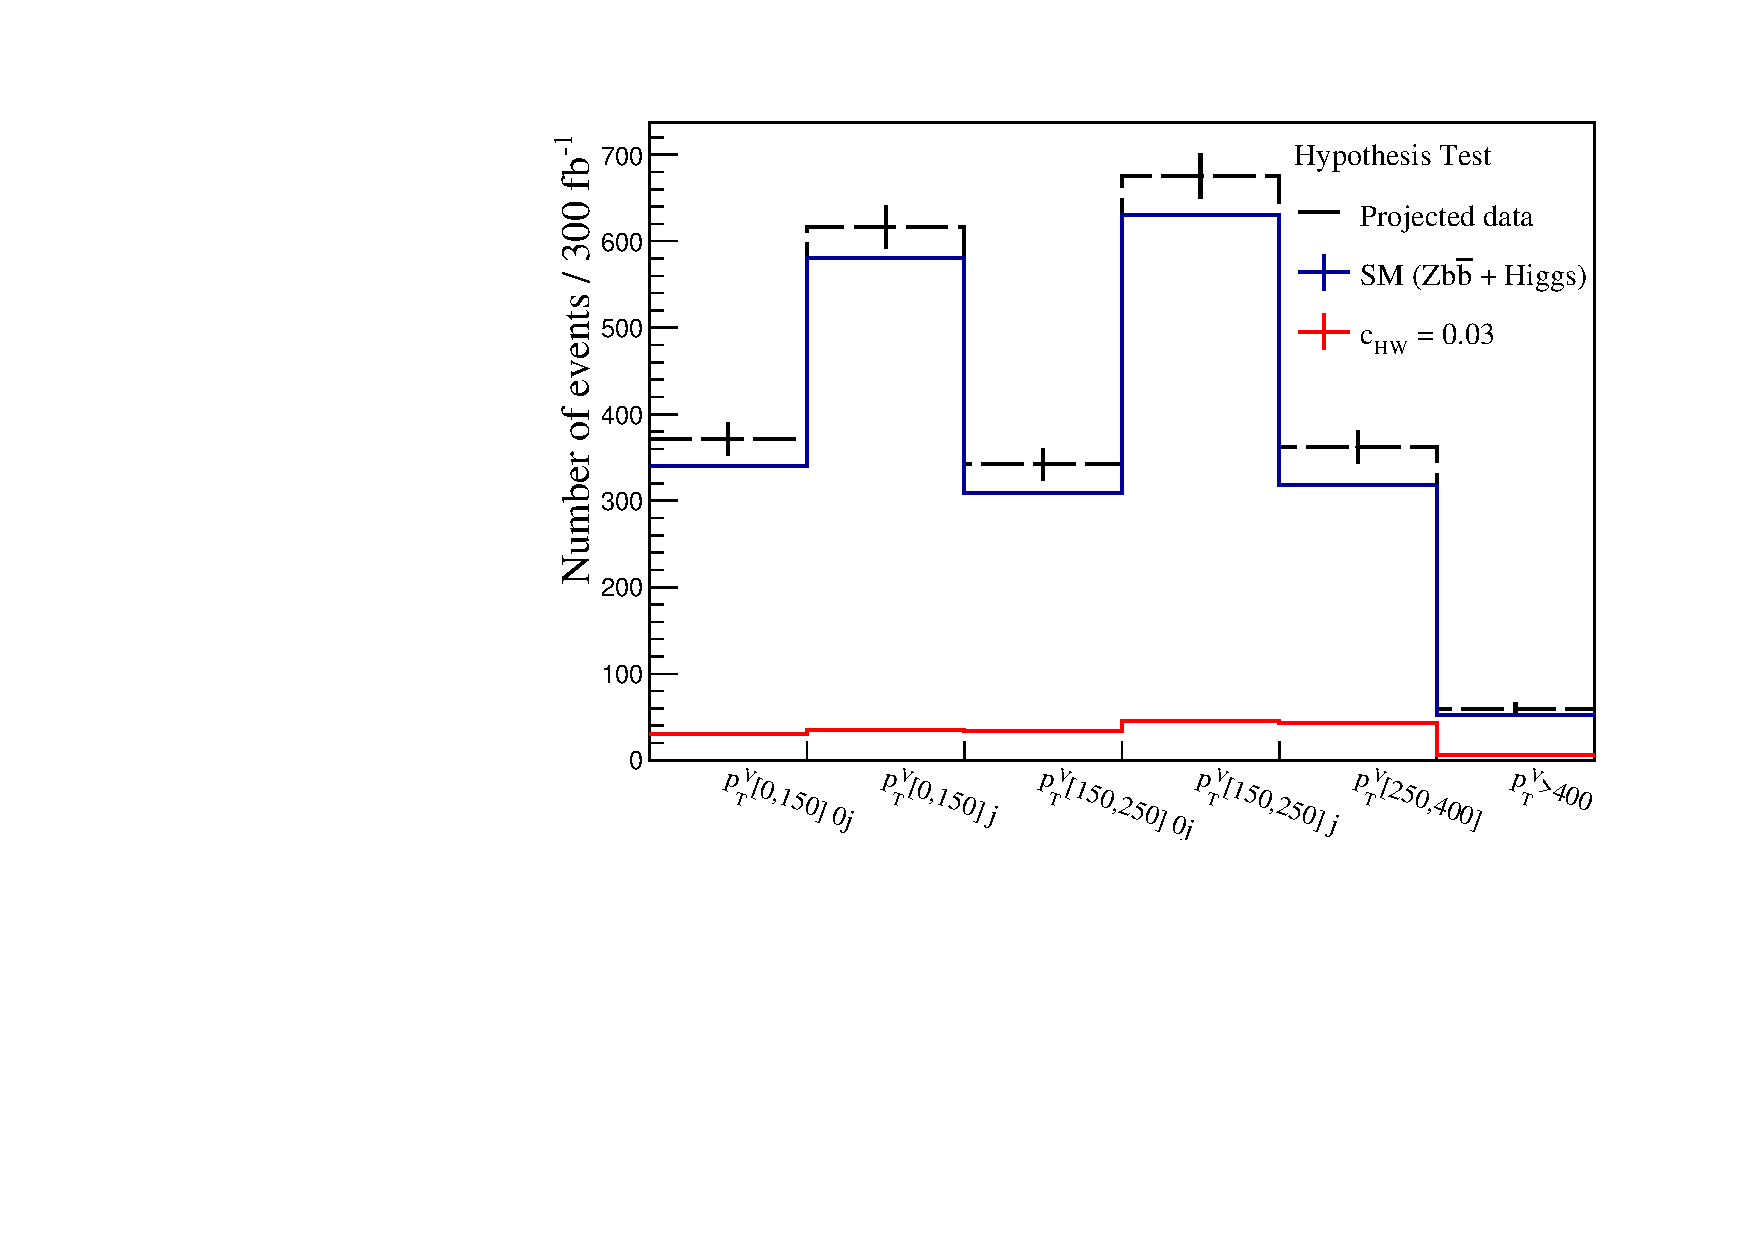
\includegraphics[width=0.45\textwidth]{plots/HypoTest_STXS.pdf}
      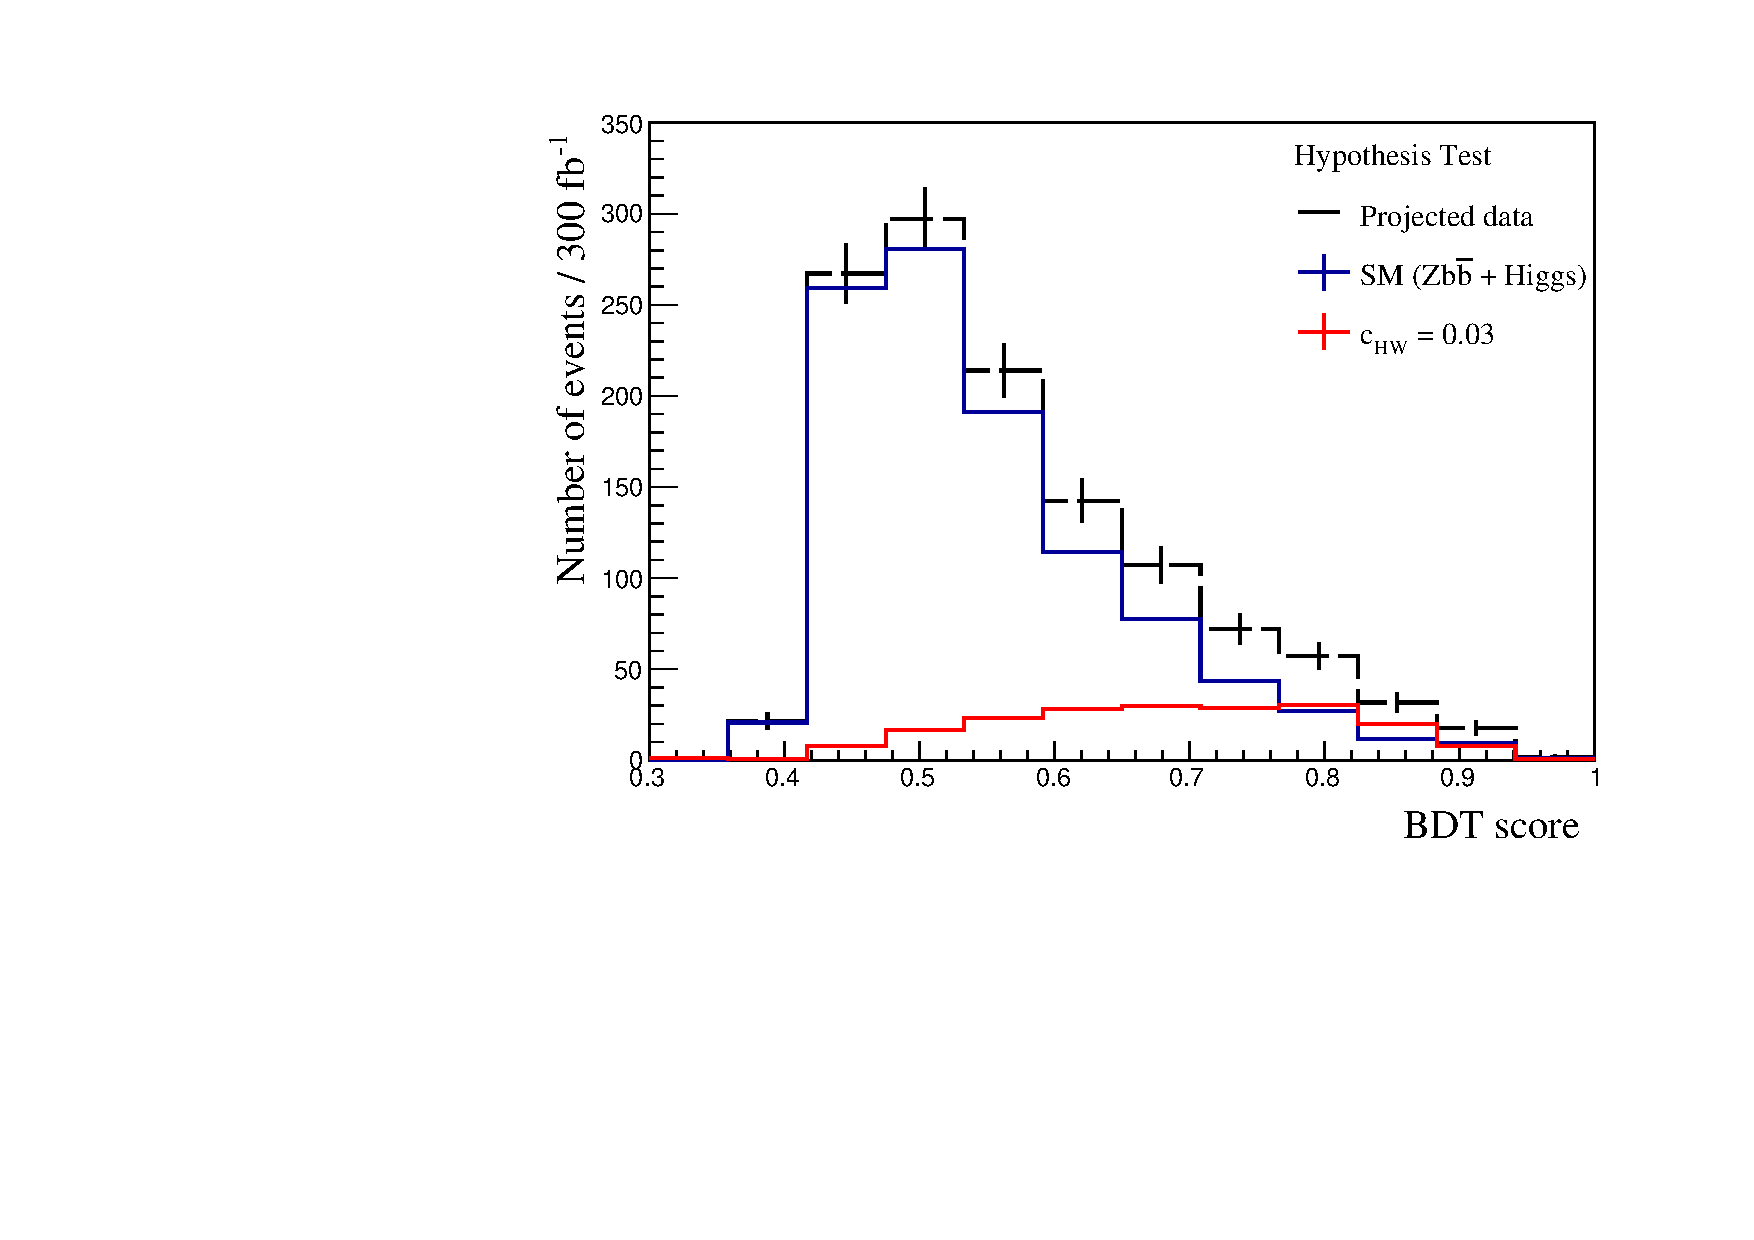
\includegraphics[width=0.45\textwidth]{plots/HypoTest_BDT.pdf}
      \caption{Predicted number of events selected for 300 fb$^{-1}$. Since the acceptance extrapolation into the STXS phase space does not change the available data statistics, it it not applied here, i.e. the distributions are shown after the first cut on the BDT classifier to reject the $Z b\bar{b}$ background.}
\label{fig:hypotest}
\end{figure}

To get a feeling of how realistic the scenario investigated herein is, the significance of a Higgs discovery in the STXS scenario is also investigated in addition to investigating the BSM sensitivity. The expected significances for the 2-lepton channel investigated here are 1.9 for ATLAS~\ref{Aaboud:2017xsd} and 1.8 for CMS~\ref{Sirunyan:2017elk} for $\sim$36 fb$^{-1}$. This is about what is expected from the simplified studies herein, which do not account for systematic uncertainties (which make up half the total uncertainty in the measurements), however are not optimized for a Higgs observation. The expected significance of a Higgs signal compared to a background (i.e. $Z b\bar{b}$) only sample is shown in Table~\ref{tab:significances}.

Table~\ref{tab:significances} also summarizes the significances found for the three luminosity scenarios for the hypothesis tests for the STXS and the BDT approach for Wilson coefficients of $c_{\sss HW} = \pm0.03$ and $c_{\sss HW} = \pm0.01$. In the case of the BDT approach and $c_{\sss HW} = \pm0.03$, three alternatives were tested. For these either the first BDT selection with the same STXS SM-acceptance or the same BDT cut as STXS are investigated and in addition a non-optimal BDT discriminant is used, that was trained not on the targeted Wilson coefficient but on it's opposite charge equivalent. 

Surprisingly, the BDT approach that dedicatedly targets the BSM encapsuled by the Wilson coefficient does perform rather similar to the STXS, independently of which $Z b\bar{b}$ rejection settings was used. As expected the usage of the non-optimal BDT discriminant reduces the expected significance significantly. The explanation might be that in $ZH$ production the kinematic correlations are very clear and evident such that the BDT fails to provide more separation power. For the smaller Wilson coefficient of $c_{\sss HW} = \pm0.01$, the BDT performs slightly better compared to the STXS, possibly because for small coefficiencts, the BDT can indeed give a slightly better separation power. This however would need to better studied. Further investigations concerning a comparison between BDT and STXS for less well-defined kinematic environments would be also interesting.


 %c_{\sss HW} = \pm 0.03 \text{ and } \pm0.01\,,

\begin{table}[!h]
\begin{center}
{\scriptsize
\begin{tabular}{|l|c|c|c|c|c|c|c|c|c|}
\hline  
Hypothesis test		&  Full Run-2 (150 fb$^{-1}$) 	& LHC Run-3 (300 fb$^{-1}$) 	& HL-LHC  (3000 fb$^{-1}$) \\ \hline

STXS: Higgs discovery	& 		3.01 &  	3.70
			& 8.06 \\ \hline

STXS: $c_{\sss HW} = 0.03$ &		6.44 	&	8.82	& 26.46\\
STXS: $c_{\sss HW} = -0.03$ &		1.66&	2.24 &  257 7.19\\
%%------------------------------
BDT: $c_{\sss HW} = 0.03$ (STXS SM-acceptance)&		 6.29&	8.58 & 25.61\\
BDT: $c_{\sss HW} = -0.03$ (STXS SM-acceptance)&		1.80&	2.44& 7.24\\ \hline
%%------------------------------
BDT: $c_{\sss HW} = 0.03$ (same BDT cut as STXS)&	6.17&	8.64 & 27.03\\
BDT: $c_{\sss HW} = -0.03$ (same BDT cut as STXS)&	1.74 &	2.08 & 7.50\\ \hline
%%------------------------------
BDT: $c_{\sss HW} = 0.03$ (alt BDT cut)		&4.40	&	6.15	&19.18\\
BDT: $c_{\sss HW} = -0.03$ (alt BDT cut)	&1.44	&	2.41	& 6.69\\ \hline
%%------------------------------
STXS: $c_{\sss HW} = 0.01$ &		2.26		&	3.04			& 8.78\\
STXS: $c_{\sss HW} = -0.01$ &		1.08		&	1.46			& 4.30\\ 
%%------------------------------
BDT: $c_{\sss HW} = 0.01$ &		2.62		&	3.07			& 8.90\\
BDT: $c_{\sss HW} = -0.01$ &		1.44		&	1.99			& 6.10\\ \hline
\end{tabular}
}
\vskip0.5truecm
\caption{Expected significances for different scenarios.}
\label{tab:significances}
\end{center}
\end{table} 
